% Epistract Conference Poster — tikzposter (A0, portrait)
\documentclass[25pt, a0paper, portrait, margin=20mm, innermargin=15mm,
  blockverticalspace=12mm, colspace=20mm]{tikzposter}

% ---------- packages ----------
\usepackage[T1]{fontenc}
\usepackage{helvet}
\renewcommand{\familydefault}{\sfdefault}
\usepackage{graphicx}
\usepackage{booktabs}
\usepackage{enumitem}
\usepackage{xcolor}
\usepackage{microtype}
\usepackage{tikz}

% ---------- figure path ----------
\graphicspath{{../paper/figures/}{figures/}}

% ---------- colors ----------
\definecolor{EpiBlue}{HTML}{1B3A5C}
\definecolor{EpiTeal}{HTML}{0E7C7B}
\definecolor{EpiGold}{HTML}{D4A843}
\definecolor{EpiLight}{HTML}{EDF2F7}
\definecolor{EpiDark}{HTML}{0D2137}

% ---------- theme ----------
\usetheme{Default}

\definecolorstyle{EpiColors}{
  \definecolor{colorOne}{named}{EpiDark}
  \definecolor{colorTwo}{named}{EpiTeal}
  \definecolor{colorThree}{named}{EpiGold}
}{
  \colorlet{backgroundcolor}{EpiLight}
  \colorlet{framecolor}{EpiBlue}
  \colorlet{blocktitlebgcolor}{EpiBlue}
  \colorlet{blocktitlefgcolor}{white}
  \colorlet{blockbodybgcolor}{white}
  \colorlet{blockbodyfgcolor}{EpiDark}
  \colorlet{titlebgcolor}{EpiDark}
  \colorlet{titlefgcolor}{white}
}
\usecolorstyle{EpiColors}

% ---------- title ----------
\title{\parbox{0.9\linewidth}{\centering\textbf{Beyond RAG:} Domain-Specific Agentic Architecture\\for Biomedical Knowledge Graph Construction}}
\author{Umesh Bhatt \enspace\textbullet\enspace \texttt{umesh@8thcross.com} \enspace\textbullet\enspace March 2026}
\institute{From GraphRAG to Epistract --- evolving latent knowledge graphs for drug discovery}

% ---------- remove tikzposter watermark ----------
\tikzposterlatexaffectionproofoff

% ===================================================================
\begin{document}

\maketitle

\begin{columns}

% ==================== LEFT COLUMN ====================
\column{0.48}

% --- MOTIVATION ---
\block{Motivation}{
  \large
  Knowledge graphs are essential for drug discovery, yet traditional construction
  requires \textbf{domain-specific models retrained per therapeutic area}.
  GraphRAG showed LLMs can extract knowledge without training, but produces
  \textbf{untyped, similarity-based edges} --- a scientist cannot distinguish
  a side effect from a mechanism of action.

  \vspace{6pt}
  \textbf{Epistract} replaces proximity with \textbf{comprehension}: parallel LLM agents
  extract typed relations against a domain schema and validate molecular identifiers
  with deterministic tools.
}

% --- ARCHITECTURE ---
\block{Architecture}{
  \centering
  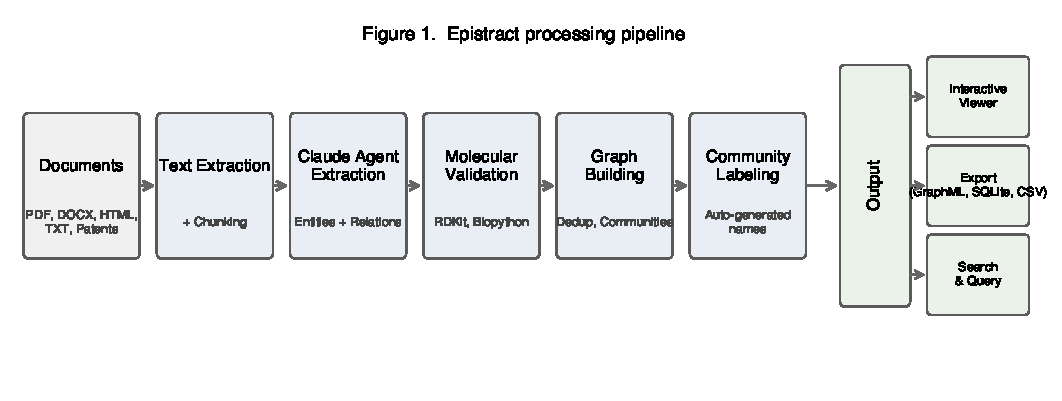
\includegraphics[width=0.90\linewidth]{fig1-architecture.pdf}

  \vspace{8pt}
  \large
  \begin{minipage}[t]{0.47\linewidth}
    \begin{itemize}[leftmargin=1.2em, itemsep=3pt, topsep=0pt]
      \item[\textcolor{EpiTeal}{\textbf{1}}] \textbf{Parallel extraction} --- one LLM agent per document
      \item[\textcolor{EpiTeal}{\textbf{2}}] \textbf{Schema enforcement} --- 17 entity types, 30 relation types
    \end{itemize}
  \end{minipage}%
  \hfill
  \begin{minipage}[t]{0.47\linewidth}
    \begin{itemize}[leftmargin=1.2em, itemsep=3pt, topsep=0pt]
      \item[\textcolor{EpiTeal}{\textbf{3}}] \textbf{Molecular validation} --- RDKit, Biopython
      \item[\textcolor{EpiTeal}{\textbf{4}}] \textbf{Graph construction} --- dedup, communities, semantic labels
    \end{itemize}
  \end{minipage}
}

% --- KEY DISTINCTION ---
\block{Comprehension vs.\ Co-occurrence}{
  \centering
  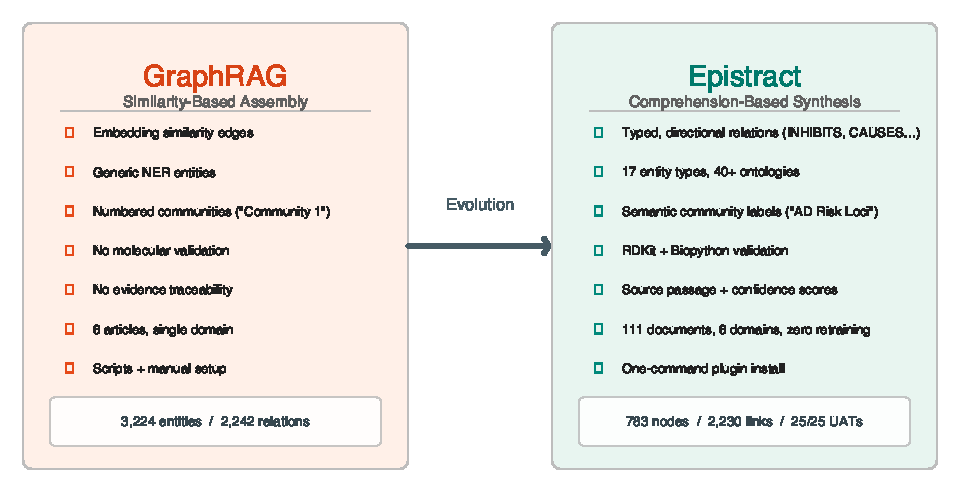
\includegraphics[width=0.85\linewidth]{fig6-evolution.pdf}
}

% --- DOMAIN SCHEMA (text only, no figure) ---
\block{Domain Schema}{
  \large
  \begin{minipage}[t]{0.46\linewidth}
    \textbf{17 Entity Types} in 6 categories:\\[4pt]
    \normalsize
    \begin{tabular}{@{}lr@{}}
      Drug \& Chemistry & 2 \\
      Molecular Biology & 5 \\
      Disease \& Phenotype & 3 \\
      Clinical & 3 \\
      Pathways \& Mechanisms & 2 \\
      Context & 2 \\
    \end{tabular}
  \end{minipage}%
  \hfill
  \begin{minipage}[t]{0.50\linewidth}
    \textbf{30 Directed Relation Types}:\\[4pt]
    \normalsize
    Drug--Target (5), Drug--Disease (2),
    Drug--Clinical (2), Drug--Drug (3),
    Molecular Biology (12),
    Biomarker (2), Organizational (3),
    Fallback (1)

    \vspace{4pt}
    Grounded in \textbf{40+ ontologies}:\\
    ChEBI, HGNC, UniProt, MeSH, MedDRA, KEGG, Reactome
  \end{minipage}
}


% ==================== RIGHT COLUMN ====================
\column{0.48}

% --- KEY RESULTS ---
\block{Evaluation: Six Drug Discovery Domains}{
  \centering

  \large
  \begin{tabular}{@{}clrrrc@{}}
    \toprule
    \textbf{\#} & \textbf{Domain} & \textbf{Docs} & \textbf{Nodes} & \textbf{Links} & \textbf{UATs} \\
    \midrule
    1 & Neurogenetics (PICALM / Alzheimer's) & 15 & 149 & 457 & 4/4 \\
    2 & Oncology (KRAS G12C inhibitors) & 16 & 108 & 307 & 5/5 \\
    3 & Rare Disease (PKU, Achondro., NPC) & 15 & 94 & 229 & 3/3 \\
    4 & Immuno-Oncology (Checkpoints) & 16 & 132 & 361 & 4/4 \\
    5 & CV / Inflammation & 15 & 94 & 246 & 3/3 \\
    6 & GLP-1 Competitive Intel.$^\dagger$ & 34 & 206 & 630 & 6/6 \\
    \midrule
      & \textbf{Total} & \textbf{111} & \textbf{783} & \textbf{2,230} & \textbf{25/25} \\
    \bottomrule
  \end{tabular}

  \vspace{2pt}
  {\normalsize $^\dagger$Multi-source: PubMed + Google Scholar + Google Patents via SerpAPI}

  \vspace{12pt}

  \begin{minipage}[c]{0.30\linewidth}
    \centering
    {\fontsize{68}{76}\selectfont\textcolor{EpiTeal}{\textbf{100\%}}}\\[2pt]
    {\large Entity Type Coverage}
  \end{minipage}%
  \hfill
  \begin{minipage}[c]{0.30\linewidth}
    \centering
    {\fontsize{68}{76}\selectfont\textcolor{EpiTeal}{\textbf{93\%}}}\\[2pt]
    {\large Relation Type Coverage}
  \end{minipage}%
  \hfill
  \begin{minipage}[c]{0.30\linewidth}
    \centering
    {\fontsize{68}{76}\selectfont\textcolor{EpiTeal}{\textbf{25/25}}}\\[2pt]
    {\large UATs Passed}
  \end{minipage}
}

% --- GRAPH VISUALIZATIONS ---
\block{Knowledge Graph Visualizations}{
  \centering
  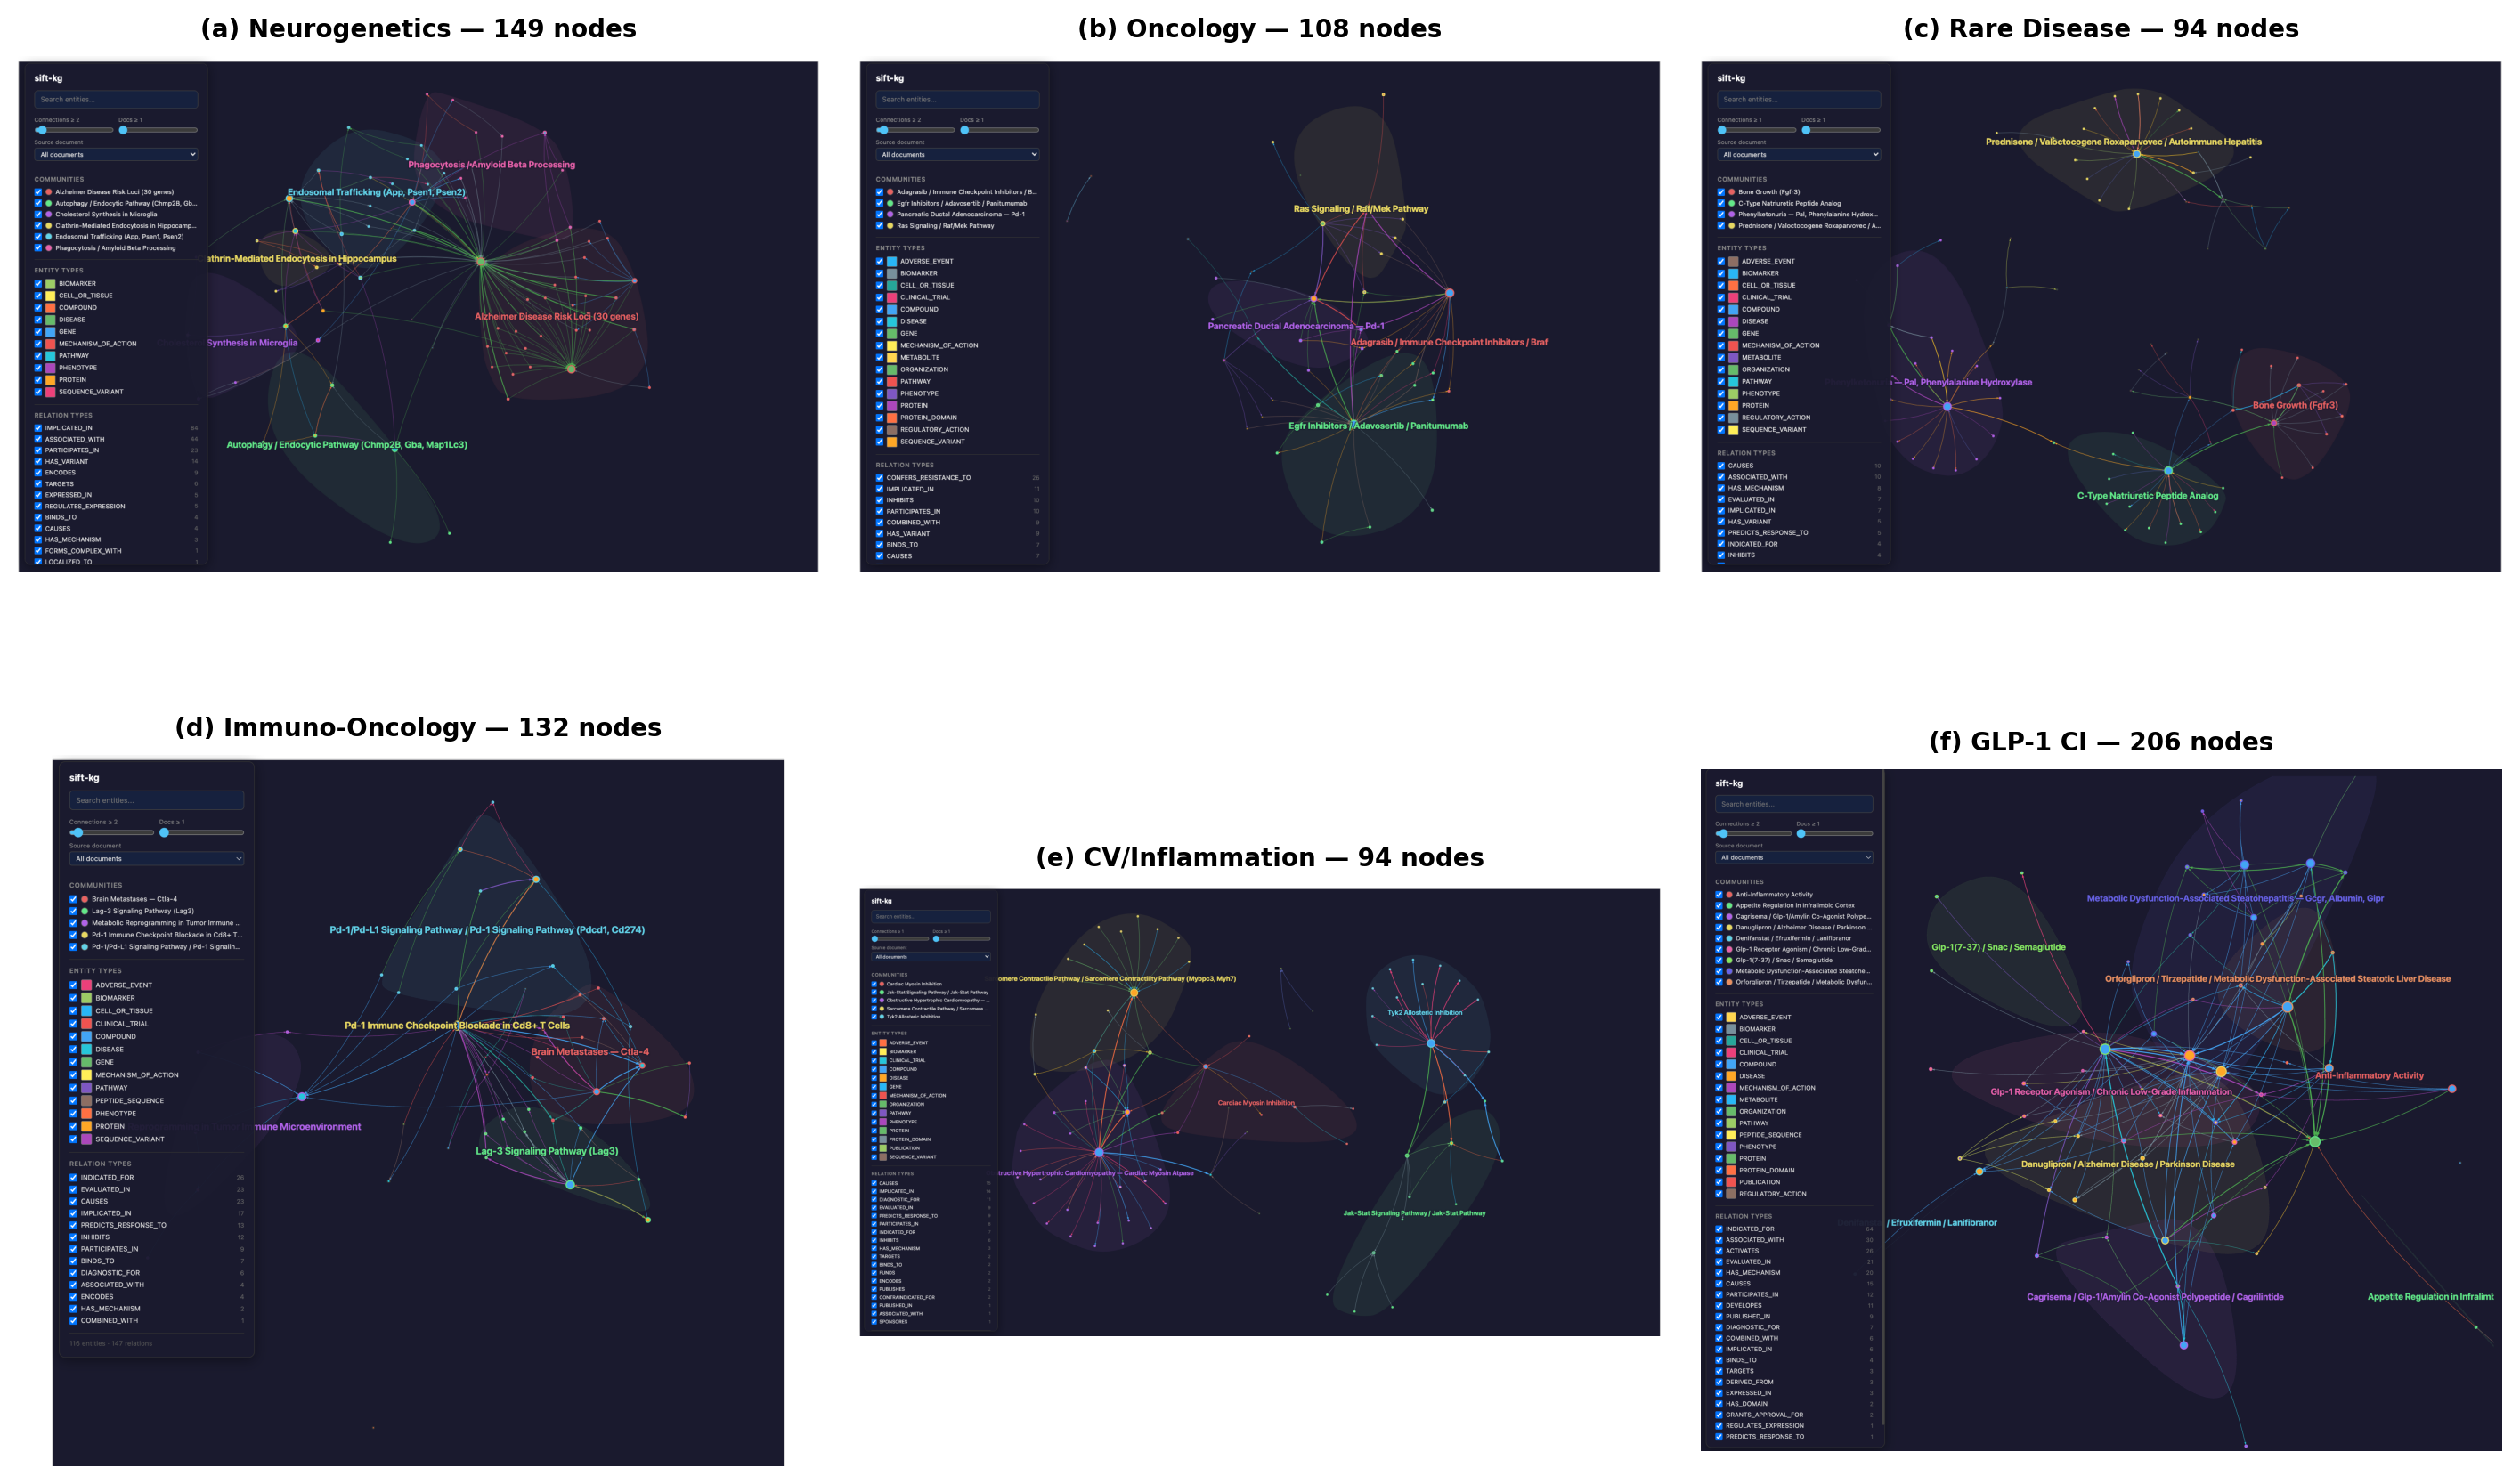
\includegraphics[width=0.92\linewidth]{fig3-scenario-graphs.png}

  \vspace{4pt}
  \large
  33 auto-labeled communities across 6 scenarios. Community detection correctly separates
  unrelated therapeutic areas and identifies commercially meaningful clusters.
}

% --- CONCLUSIONS ---
\block{Key Contributions}{
  \large
  \begin{itemize}[leftmargin=1.2em, itemsep=4pt, topsep=0pt]
    \item \textbf{Method:} Agentic extraction with typed domain schemas, parallel agent dispatch,
      and molecular validation (RDKit + Biopython)
    \item \textbf{Tool:} Open-source Claude Code plugin, installable in one command,
      with all test corpora and outputs committed for reproducibility
    \item \textbf{Multi-source:} PubMed + Google Scholar + Google Patents ---
      mirrors how human researchers conduct competitive intelligence
  \end{itemize}
}

\end{columns}

% ---------- FOOTER (as a full-width block) ----------
\block[titlewidthscale=1.0, bodywidthscale=1.0]{}{
  \centering
  \large
  \textbf{Open Source} \textbullet{} MIT License \textbullet{}
  \texttt{github.com/usathyan/epistract}\\[4pt]
  Install: \texttt{claude plugin install epistract}
}

\end{document}
